\begin{frame}[fragile]{整体内容}
  \begin{easylist} \easyitem
    & 简介
    & 数据类型
    & 控制流
    & 函数
    & 模块
    & 标准库
    & 面向对象编程
    & 异常、调试与测试
    & 输入输出
    & 应用(Web, DB, etc.)
  \end{easylist}
\end{frame}


\begin{frame}[fragile]{致谢}
  \begin{easylist}
    & 本课件的制作参考了部分图书和第三方网络资源,在此对原作者表达致谢和敬意,如
    有侵权需要从本课件中移除,请留言或联系xiat(at)ruc.edu.cn。参考资料包括但不限
    于以下:
    && 廖雪峰,
    \href{http://www.liaoxuefeng.com/wiki/0014316089557264a6b348958f449949df42a6d3a2e542c000}{Python教程}
    && Introducing Python by Bill Lubanovic
    && Dive Into Python 3 by Mark Pilgrim
    && Magnus Lie Hetland, 司维等翻译,Python基础教程(2ed), 人民邮电出版社
    && NumPy Cookbook
    && Python for Data Analysis
  \end{easylist}

\end{frame}

\section{引论}

\begin{frame}[fragile]{CH1 简介}
  \begin{easylist} \easyitem
    & 1.1 什么是Python
    & 1.2 Python可以做什么
    & 1.3 如何安装Python
    & 1.4 Python开发环境
    & 1.5 如何运行Python程序
    & 1.6 若干例子
  \end{easylist}
\end{frame}

\begin{frame}[fragile]{You're flying!}
  \begin{center}
    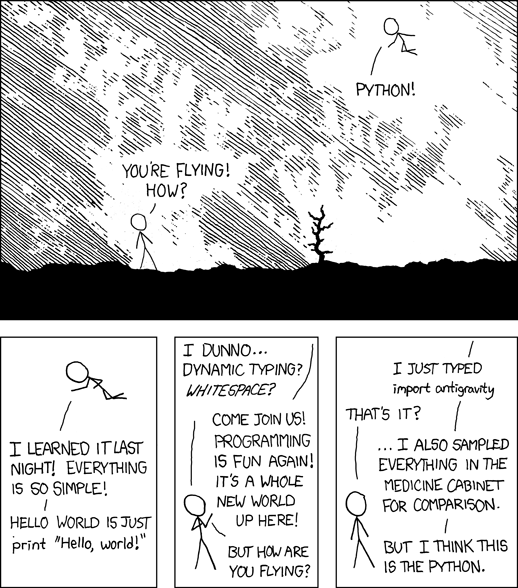
\includegraphics[height=0.9\textheight]{figure/fly.jpg}
  \end{center}
\end{frame}

\begin{frame}[fragile]{用Python,飞一般的感觉!}
  \begin{easylist}
    & \color{red} Friend :“你在飞!怎么做到的?”
    & Cueball:“Python!我昨晚刚刚学会了Python。一切都变得如此简单!写一个Hello World 程序只要一行代码 print "Hello World!" 就搞定了!”
    & \color{red}Friend :“ 什么情况?呃……动态类型?泛空格符?”
    & Cueball:“来加入我们吧,有了Python,编程再次变得有趣。这是一个全新的世界!”
    & \color{red}Friend :“但是你到底是怎么飞在天上的?”
    & Cueball:“我只是输入了“import antigravity” 命令而已。”
    & \color{red}Friend :“就这样?”
    & Cueball:“我还把药柜中的药嗑了个遍……但我觉得还是 Python 的原因。”
  \end{easylist}
\end{frame}

\begin{frame}[fragile]{1.1 什么是Python}
  \begin{easylist}
    & Python是一种既简单又强大的编程语言
    & 注重如何解决问题,而不是编程语言的语法和结构
    & 拥有高效的高级数据结构,简单有效地实现面向对象编程
    & 语法简洁、动态解释、适用于快速应用开发和脚本编程
    & 在数据科学中大有用武之地
  \end{easylist}
\end{frame}

\begin{frame}[plain]{}
  \begin{tikzpicture}[remember picture,overlay]
    \node[xshift=-60, yshift=-60] at (current page.north east) {
\includegraphics[]{figure/tim.png} };
  \end{tikzpicture}

  \LARGE The Zen of Python, \small by Tim Peters

  \normalsize 
  Beautiful is better than ugly. \\
  Explicit is better than implicit. \\
  Simple is better than complex. \\
  Complex is better than complicated. \\
  Flat is better than nested. \\
  Sparse is better than dense. \\
  Readability counts. \\
  Special cases aren't special enough to break the rules. \\
  Although practicality beats purity. \\
  Errors should never pass silently. \\
  Unless explicitly silenced.\\
  In the face of ambiguity, refuse the temptation to guess.\\
  There should be one-- and preferably only one --obvious way to do it.\\
  Although that way may not be obvious at first unless you're Dutch.\\
  Now is better than never.\\
  Although never is often better than *right* now.\\
  If the implementation is hard to explain, it's a bad idea.\\
  If the implementation is easy to explain, it may be a good idea.\\
  Namespaces are one honking great idea -- let's do more of those!\\
\end{frame}

\begin{frame}[plain]{}
  \begin{tikzpicture}[remember picture,overlay]
    \node[xshift=-60, yshift=-60] at (current page.north east) {
\includegraphics[]{figure/tim.png} };
  \end{tikzpicture}

  \LARGE Python之禅 \small by Tim Peters

  \normalsize
  优美胜于丑陋 \\ {\tiny Python 以编写优美的代码为目标}\\
  明了胜于晦涩 \\ {\tiny 优美的代码应当是明了的,命名规范,风格相似}\\
  简洁胜于复杂 \\ {\tiny 优美的代码应当是简洁的,不要有复杂的内部实现}\\
  复杂胜于凌乱 \\ {\tiny 如果复杂不可避免,那代码间也不能有难懂的关系,要保持接口简洁}\\
  扁平胜于嵌套 \\ {\tiny 优美的代码应当是扁平的,不能有太多的嵌套}\\
  间隔胜于紧凑 \\ {\tiny 优美的代码有适当的间隔,不要奢望一行代码解决问题}\\
  可读性很重要 \\ {\tiny 优美的代码是可读的}\\
  即便假借特例的实用性之名,也不可违背这些规则 \\ {\tiny 这些规则至高无上} \\
  不要包容所有错误,除非你确定需要这样做 \\ {\tiny 精准地捕获异常,不写 except:pass 风格的代码}\\
  当存在多种可能,不要尝试去猜测\\
  而是尽量找一种,最好是唯一一种明显的解决方案({\tiny 如果不确定,就用穷举法})\\
  虽然这并不容易,因为你不是 Python 之父({\tiny 这里的 Dutch 是指 Guido})\\
  做也许好过不做,但不假思索就动手还不如不做({\tiny 动手之前要细思量})\\
  如果你无法向人描述你的方案,那肯定不是一个好方案;反之亦然(方案测评标准)\\
  命名空间是一种绝妙的理念,我们应当多加利用(倡导与号召)\\
\end{frame}

\begin{frame}[fragile]{编程语言排名@Feb, 2016}
  \begin{easylist}
    & Java
    & C
    & C++
    & C\#
    & \em Python $\star$
    & PHP
    & Visual Basic
    & Perl
    & JavaScript
    & Delphi/Object Pascal
  \end{easylist}
  From: \url{http://www.tiobe.com/tiobe_index?page=index}
\end{frame}


\begin{frame}[fragile]{1.2 Python可以做什么}
  \begin{easylist}
    & Almost anything
    && From system management, security, web, \\
    to data mining, machine learning ...
    & 数据科学界华山论剑:R与Python巅峰对决 \\
    \url{http://chuansong.me/n/1458679}
    & 为什么很多人喜欢 Python? \\
    \url{https://www.zhihu.com/question/28676107}
  \end{easylist}
\end{frame}

\begin{frame}[fragile]{一段简单的Python代码}
~
  \begin{python}
    #Python 3: Fibonacci series up to n
    def fib(n):
        a, b = 0, 1
        while a < n:
            print(a, end=', ')
            a, b = b, a+b
        print()
    fib(100)
  \end{python}
  Result: 0, 1, 1, 2, 3, 5, 8, 13, 21, 34, 55, 89, 

\end{frame}


\begin{frame}[fragile]{1.3 如何安装Python}
  \begin{easylist}
    & 在线直接编写运行
    && Host, run, and code Python in the cloud!
    && https://www.python.org/
    & python shell及增强版本
    & 编辑器编辑代码文件,利用python运行
  \end{easylist}
\end{frame}

\begin{frame}[fragile]{Python shell}
  \begin{bash}
    $python3
    Python 3.4.3+ (default, Oct 14 2015, 16:03:50) 
    [GCC 5.2.1 20151010] on linux
    Type "help", "copyright", "credits" or "license" for more information.
    >>> 
  \end{bash}
\end{frame}

\begin{frame}[fragile]{课堂练习}
  \begin{easylist}
    & Windows环境下Python程序的安装和运行测试
    && https://www.python.org/downloads/
    & 注意:本课程后续讲解均以Linux(Ubuntu)作为操作系统环境
  \end{easylist}
\end{frame}

\begin{frame}[fragile]{安装EasyInstall}
  \begin{easylist}
    & wget\textvisiblespace http://peak.telecommunity.com/dist/ez\_setup.py
    & python\textvisiblespace ez\_setup.py\textvisiblespace setuptools
    & ez\_install\textvisiblespace pip
    & ez\_install\textvisiblespace pip3
  \end{easylist}
\end{frame}

\begin{frame}[fragile]{Python2 vs Python3}
  \begin{easylist}
    & Python3是Python2的重大变更版本
    & 有许多正在运行的程序使用了Python2
    & 系统中可以同时安装python2和python3
    & 与Python2相比,Python3相关的工具多以3结尾,如ipython3
    & 本课程讲解以Python3为主,穿插Python2的语法
  \end{easylist}
\end{frame}


\begin{frame}[fragile]{1.4 Python开发环境}
  \begin{easylist}
    & Python shell
    && 自带的命令解释器
    && ipython
    && jupyter notebook
    && bpython
    & Editor
    && pycharm
    && Sublime text
    && Emacs
    && Vim
  \end{easylist}
\end{frame}

\begin{frame}[fragile]{ipython}
  \begin{easylist}
    & sudo\textvisiblespace apt-get\textvisiblespace install\textvisiblespace ipython3
    & 展示
  \end{easylist}
\end{frame}

\begin{frame}[fragile]{bpython}
  \begin{easylist}
    & sudo\textvisiblespace apt-get\textvisiblespace instal\textvisiblespace bpython3
    & 展示
  \end{easylist}
\end{frame}

\begin{frame}[fragile]{善用help}
  利用Python自带的help函数获取帮助

  \pyinline{help(max)}

  \pyinline{help()}
\end{frame}

\begin{frame}[fragile]{增强命令行}
  \begin{easylist}
    & tmux
    & zsh
  \end{easylist}
\end{frame}


\begin{frame}[fragile]{1.5 如何运行Python程序}
  \begin{easylist}
    & 直接在Python Shell中输入,解释执行
    & 保存到文件中,以.py结尾,通过python运行
    && 如把前面的斐波那契数列的代码保存到文本文件中,并把文件名命名为fib.py
    && python3\textvisiblespace fib.py
    \pause
    & 可执行的Python脚本
    && 在Python脚本文件的开头加上一行声明 
    &&& \#!/usr/bin/python3
    &&& chmod u+x filename.py
  \end{easylist}
\end{frame}

\begin{frame}[fragile]{代码清单:fib.py}
  \lstinputlisting[keywordstyle=\ttfamily]{src/fib.py}
\end{frame}

\begin{frame}[fragile, allowframebreaks]{1.6 一个完整的Python程序}
  \lstinputlisting[keywordstyle=\ttfamily, basicstyle=\rmfamily\normalsize]{src/humansize.py}
  Code From: ``Dive into Python 3''
\end{frame}

\begin{frame}[fragile]{例子解释}
  \begin{easylist}
    & 如何声明函数:def
    & 可选的和命名的参数
    & 文档字符串
    & 代码缩进
    & 异常
    & 大小写  
  \end{easylist}
\end{frame}

\begin{frame}[fragile]{Python基本用法预览}
  \begin{easylist}
    & 把Python当做计算器
    & 字符串的表示
    & 字符串切片
  \end{easylist}
\end{frame}

\begin{frame}[fragile]{把Python当做计算器}
  \begin{easylist}
    & Python解释器可以当做简单的计算器,输入表达式,即可对表达式求值
    & 练习
    && 打开Python解释器,输入以下表达式求值
    && 2+2
    && 8/5 \#结果是1.6? 还是1? %默认不会丢失小数部分
    && (3+5)/2
    && 8//5 %相当于整除 
  \end{easylist}
\end{frame}

\begin{frame}[fragile]{字符串的表示}
  \begin{easylist}
    & 单引号
    & 双引号
    & 三引号
  \end{easylist}
  \begin{python}
    msg = 'hello "Python"'
    print(msg)
    msg = "hello 'Python'"
    print(msg)
    msg = '''
        hello
        world!
        '''
    print(msg)
  \end{python}
\end{frame}


\begin{frame}[fragile]{字符串切片}
    $>>>$ msg = '中国人民大学信息资源管理学院'

    $>>>$ msg[0] \\ '中'

    $>>>$ msg[-8:-1] \\ '信息资源管理学'

    $>>>$ ms g[-8:] \\ ??

    $>>>$ msg[:6] 

    $>>>$ msg[:]
\end{frame}


\begin{frame}[fragile]{---END---}
  \begin{center}
    \Simley{1}{10}{1}
  \end{center}
\end{frame}

%%% Local Variables:
%%% mode: latex
%%% TeX-master: "../python"
%%% End:
